\section{Planning by Dynamic Programming}

\subsection{Introduction: Dynamic Programming}
\red{Dynamic} \blue{programming} = \blue{Optimization method} for \red{sequential} problem

Breaks down complex problem into subproblems, solves subproblems, combines solutions of the subproblems. Useful when problems have two properties:
\begin{itemize}
	\item optimal \underline{sub}structure: solving smaller subproblems helps to solve original problem
	\item overlapping subproblems: subproblems appear many times and caching of results helps
\end{itemize}

MDP satisfies both properties:
\begin{itemize}
	\item Bellman equation gives optimal substructure (recursive decomposition of problem solution into subproblems' solutions)
	\item ValueFunction is a cache for subproblem solutions.
\end{itemize}

DynProg can be applied to: 
\begin{itemize}
	\item Policy Evaluation: given the policy, how good is it?
	\item Policy Iteration: finds a good policy by working in policy space and in for loop uses Policy Evaluation
	\item Value Iteration: directly works in Value-function space and applies Bellman Equation iteratively
\end{itemize}


DynProg assumes \underline{full knowledge of MDP}, so it is only used for \textit{planning}:
\begin{itemize}
	\item for prediction: given $\MDP=<\States, \Actions, \Reward, \TransitionProb, \gamma>$ (or induced $\MRP=<\States, \Reward_\pi, \TransitionProb_\pi, \gamma>$) and a policy $\pi$, output value function $V_\pi$
	\item for control: given $\MDP=<\States, \Actions, \Reward, \TransitionProb, \gamma>$, output optimal value function $V_{*}$ and optimal policy $\pi_*$
\end{itemize}

\subsection{Policy Evaluation}
Problem: evaluate a policy $\pi$ to get $V_\pi$

Solution: start with any value function $v_0$ (e.g. all zeros) and iteratively apply Bellman expectation equation in \textit{synchronous backups}: $v_0 \to v_1 \to v_2 \to ... \to \red{v_\pi}$.

\textit{Synchronous backups}: compute $v_{k+1}(s)$ all states (in any order or even in parallel) only using previous table $v_{k}(s)$.


\begin{figure}[ht]
	\begin{minipage}{0.5\textwidth} % left column
\begin{align*}
	v_{k+1}(s) &= \sum_{a\in \Actions}  \pi(a|s) \left(\Reward_s^a + \gamma \sum_{s' \in \States} \TransitionProb_{s s'}^a v_{k}(s')\right) \\
	v^{k+1} &= \Reward^\pi + \gamma \TransitionProb^{\pi} v^k  \text{(vector form)} \notag	
\end{align*}
	\end{minipage}%
	\begin{minipage}{0.5\textwidth} % right column
	\centering
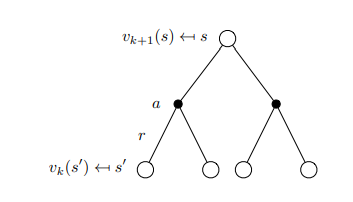
\includegraphics[width=0.6\linewidth]{img/dynprog_eval_sync_backup_tree}
\label{fig:dynprogevalsyncbackuptree}
	\end{minipage}
\caption{Synchronous backup using iterative Bellman expectation equation for policy evaluation}
\end{figure}


\begin{figure}[h]
	\centering
	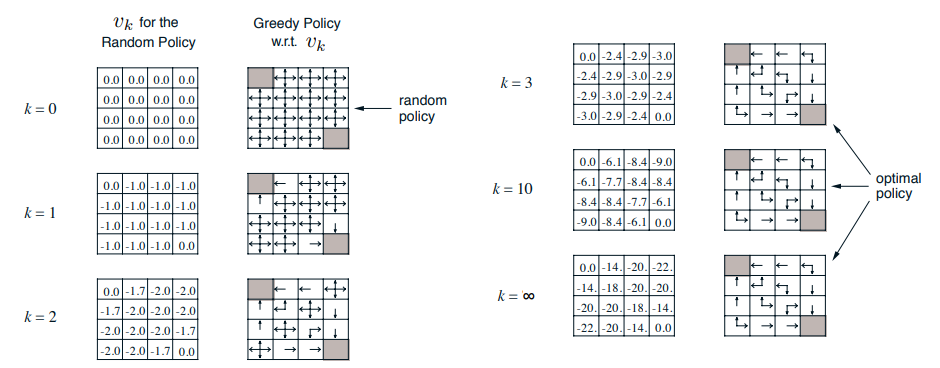
\includegraphics[width=1\linewidth]{img/dynprog_evaluation_random_policy}
	\caption{\orange{This example demonstrates important intuition that during iterations of policy evaluation we get improved policy (right column) and we see improvements in the first iterations, not waiting for convergence}}
	\label{fig:dynprogevaluationrandompolicy}
\end{figure}


\subsection{Policy Iteration}
Intuition: Given a policy $\pi$, how can we get another policy that is certainly better? And if we have such possibility, we can just iterate until convergence.